% !TeX root = ../thuthesis-example.tex

\chapter{基于图结构的RNN及其网络流量异常检测算法}

\section{引言}
% Recurrent network的应用主要如下两部分:

% 文本相关。主要应用于自然语言处理(NLP)、对话系统、情感分析、机器翻译等等领域,Google翻译用的就是一个7-8层的LSTM模型。
% 时序相关。就是时序预测问题(timeseries),诸如预测天气、温度、包括个人认为根本不可行的但是很多人依旧在做的预测股票价格问题
% 这些问题都有一个共同点,就是有先后顺序的概念的。举个例子: 根据前5天每个小时的温度,来预测接下来1个小时的温度。典型的时序问题,温度是从5天前,一小时一小时的记录到现在的,它们的顺序不能改变,否则含义就发生了变化;再比如情感分析中,判断一个人写的一篇文章或者说的一句话,它是积极地(positive),还是消极的(negative),这个人说的话写的文章,里面每个字都是有顺序的,不能随意改变,否则含义就不同了。

% 全连接网络Fully-Connected Network,或者卷积神经网络Convnet,他们在处理一个sequence(比如一个人写的一条影评),或者一个timeseries of data points(比如连续1个月记录的温度)的时候,他们缺乏记忆。一条影评里的每一个字经过word embedding后,被当成了一个独立的个体输入到网络中;网络不清楚之前的,或者之后的文字是什么。这样的网络,我们称为feedforward network。

% 但是实际情况,我们理解一段文字的信息的时候,每个文字并不是独立的,我们的脑海里也有它的上下文。比如当你看到这段文字的时候,你还记得这篇文章开头表达过一些关于LSTM的信息;

% 所以,我们在脑海里维护一些信息,这些信息随着我们的阅读不断的更新,帮助我们来理解我们所看到的每一个字,每一句话。这就是RNN的做法:维护一些中间状态信息。
% \section{网络流量的时空特性}

% \section{基于图结构的RNN原理}
% 神经网络是目前计算机科学最流行的算法之一,它在图像识别、语音识别和自然语言处理等领域取得了重大突破。卷积神经网络、循环神经网络。
\section{神经网络}

神经网络(Neural Network,NN),又称人工神经网络(Artificial Neural Network,ANN),是20世纪80 年代以来人工智能领域兴起的研究热点。它的定义有很多,其中第一批神经计算机的发明者Robert Hecht-Nielsen博士对神经网络的定义是“ 一个由许多简单的,高度互连的处理元素组成的计算系统, 它们通过对外部输入的动态状态反应来处理信息。或者也可以认为人工神经网络是一种计算模型,它的灵感来自于人脑中生物神经网络处理信息的方式。”
最近十多年来,针对人工神经网络的研究工作已经取得了重大进展,其在模式识别、自动控制、预测估计等领域已成功地解决了许多现代计算机难以解决的实际问题。

\subsection{神经网络的类型}
神经网络有很多类,这些类也有子类,最常用的类有如下几种。
\begin{enumerate}
    \item 前馈神经网络.
前馈神经网络是一种人工神经网络,单元之间的连接不形成循环。在这种网络中,信息只有一个方向,即向前移动,从输入节点,通过隐藏节点(如果有的话),然后到输出节点。网络中不存在循环或环路。
我们可以区分两种类型的前馈神经网络。
\begin{enumerate}
    \item 单层感知器。
    这是最简单的前馈神经网络,不包含任何隐藏层,也就是说它只由单层的输出节点组成。之所以说是单层,是因为我们在计算层数的时候,并不包括输入层,原因是在输入层没有进行计算,输入通过一系列的权重直接反馈给输出。
    \item 多层感知器(MLP)。
这类网络由多层计算单元组成,通常以前馈方式相互连接。一层中的每个神经元都与后一层的神经元有定向连接。在许多应用中,这些网络的单元应用一个sigmoid函数作为激活函数。MLP是非常有用的,一个很好的原因是,它们能够学习非线性表示(大多数情况下,呈现给我们的数据是不可线性分离的。
\item  卷积神经网络(CNN)。
卷积神经网络与普通的神经网络非常相似,它们是由具有可学习权重和偏差的神经元组成的。在卷积神经网络(CNN,或ConvNet或移位不变或空间不变)中,单元连接模式的灵感来自于视觉皮层的组织,单元在一个被称为感受场的受限空间区域内对刺激做出反应。感受场部分重叠,覆盖了整个视场。单元响应可以用卷积运算在数学上近似。它们是多层感知器的变体,使用最少的预处理。它们的广泛应用是在图像和视频识别,推荐系统和自然语言处理。CNNs需要大量的数据来进行训练。
\end{enumerate}
\item  循环神经网络
在循环神经网络(RNN)中,单元之间的连接形成了一个定向循环(它们向前传播数据,同时也向后传播数据,从较后的处理阶段到较早的阶段)。这使得它能够表现出动态的时间行为。与前馈神经网络不同,RNNs可以利用其内部存储器处理任意输入序列。这使得它们适用于未分割、连接的手写识别、语音识别和其他一般序列处理器等任务。
\end{enumerate}


神经网络的灵感来自于人脑生物神经网络的处理方式。
大脑的基本计算单位是神经元。在人类的神经系统中,大约有860亿个神经元,它们与大约$10^{14}$-$10^{15}$的突触相连。神经网络的基本计算单位也是神经元,通常称为节点或单位。它从其他一些节点或外部源接收输入,并计算输出。每个输入都有一个相关的权重(w),该权重是根据其对其他输入的相对重要性分配的。节点对其输入的加权和应用一个函数。
其想法是,突触强度(权重w)是可学习的,并控制影响的强度及其方向:一个神经元对另一个神经元的兴奋性(正权重)或抑制性(负权重)
% 。在基本模型中,树突将信号传到细胞体,在那里它们都会被相加。如果最后的总和超过了某个阈值,神经元就可以开火,沿着轴突发出一个尖峰。在计算模型中,我们假设尖峰的精确时序并不重要,只有发射的频率能传递信息。我们用激活函数(e.x sigmoid函数)来模拟神经元的发射率,它代表沿轴突的尖峰频率。
% 开火 TODO
% 从上面的解释我们可以得出结论,神经网络是由神经元组成的,生物学上神经元是通过突触连接的,信息在突触中流动(出计算模型的权重),当我们训练一个神经网络时,我们希望神经元每当从数据中学习到特定的模式时就开火,我们用激活函数来模拟开火率。

假设一个神经元接收$𝐷$ 个输入$x_1,x_2,...,x_D$令向量$x=[x_1;x_2;...;x_D]$来
表示这组输入, 净输入也叫净活性值
(Net Activation).
并用净输入(Net Input)$z\in \mathbb{R}$表示一个神经元所获得的输入信
号$x$的加权和,

\begin{equation}
\begin{aligned}    
    z &= \sum_{d=1}^D w_d x_d + b \\
      &= w^Tx + b        
\end{aligned}    
\end{equation}

其中$w=[w_1;w_2;...;w_D] \in \mathbb{R}^D$ 是$𝐷$ 维的权重向量,$b\in \mathbb{R}$是偏置。


净输入$𝑧$在经过一个非线性函数$f(\cdot)$后,得到神经元的活性值(Activation,
\begin{equation}
    a = f(z)
\end{equation}
其中非线性函数$f(\cdot)$称为激活函数。

一个人工神经元的结构如图~\ref{fig:神经元}所示:
\begin{figure}
    \centering
    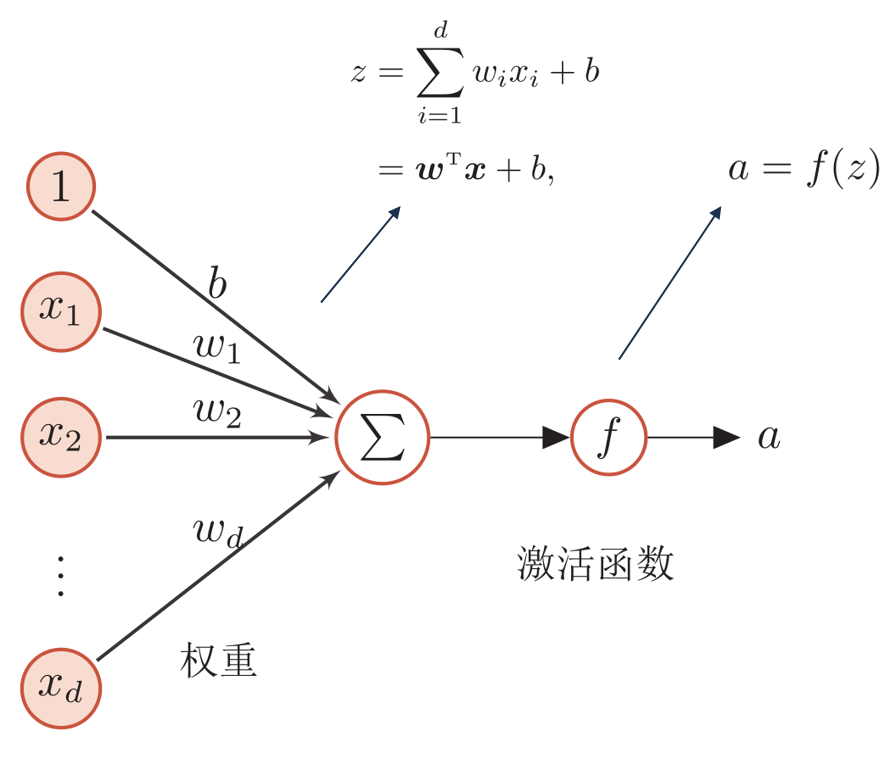
\includegraphics[width=0.6\linewidth]{人工神经元.png}
    \caption{人工神经元模型}
    \label{fig:神经元}
  \end{figure}

在图~\ref{fig:神经元}中,$\vec{x}$为输入向量,$w$和$b$分别是权重和偏移,

神经网络主要由以下几部分组成:
\begin{itemize}
    \item 输入节点(输入层)。在这一层中不进行任何计算,它们只是将信息传递给下一层(大部分时间是隐藏层)。
    \item 隐藏节点(隐藏层)。中间处理或计算在隐藏层中完成的,然后将输入层的权重(信号或信息)传递给下一层(另一个隐藏层或输出层)。一个神经网络也可以不包含隐藏层。
    \item 输出节点(输出层)。它是神经网络的最后一层,接收来自最后一个隐藏层的输入。通过激活函数可以得到合理范围内的理想数值,例如用于分类的softmax函数。
    \item 连接和权重。神经元之间会有边进行连接,每条边会有一定的权重。即每个连接将神经元$i$的输出传递给神经元$j$的输入,每个连接被赋予一个权重$W_{ij}$。
    \item 激活函数。激活函数负责为神经网络引入非线性特征。它把值压缩到一个更小范围,即一个 Sigmoid 激活函数的值区间为 [0,1]。深度学习中有很多激活函数,如Sigmoid、Tanh、ReLU 、Softplus、Softmax 等。下表为常见的激活函数。
    \begin{table}[]
        \caption{激活函数}
        \centering
        \begin{tabular}{|l|l|l|}
        \hline
        名称&表达式&导数\\ \hline
        Sigmoid &  $f(x) = \frac{1}{1+e^{-x}}$ & $f'(x) = f(x)(1-f(x))$
        \\ \hline
        Tanh & $f(x) = \frac{2}{1+e^{-2x}} - 1$ & $f'(x) = 1 - f(x)^2$ \\ \hline
        ReLU & $f(x) = max(0, x)$ & $f(x)=\begin{cases}
        0& \text{x<0}\\
        1& \text{x>=0}
        \end{cases}$ \\ \hline
        Softplus & $f(x) = log(1+e^x)$ & $f'(x) = \frac{1}{1+e^x}$ \\ \hline
        Softmax & $S_i = \frac{e_i}{\sum_j e_j}$ & \\ \hline
        \end{tabular}
        \end{table}
    \item 学习规则。学习规则是一种规则或算法,它修改神经网络的参数,以使网络的给定输入产生一个有利的输出。这个学习过程通常相当于修改权重和阈值。
\end{itemize}

\subsection{RNN}
RNN是一种针对时序数据处理的神经网络模型。相较于普通的神经网络模型来说,更擅长处理序列数据,即该网络其具有短期记忆能力。在循环神经网络中,神经元不但可以接受其他神经元的信息,也可以接受自身的信息,形成具有环路的网络结构。
% 神经网络有很多类型,这里本文将神经网络划分为前馈神经网络和循环神经网络,其中前馈神经网络包含单层感知机、多层感知机(MLP)、卷积神经网络(CNN)等。
% 本文主要介绍循环神经网络, 循环神经网络(Recurrent Neural Network,RNN)是一类具有短期记忆能力的神经网络。.和前馈神经网络相比,循环神经网络更加符合生物神经网络的结构。
下图~\ref{fig:循环神经网络}是循环神经网络的示意图。
\begin{figure}
    \centering
    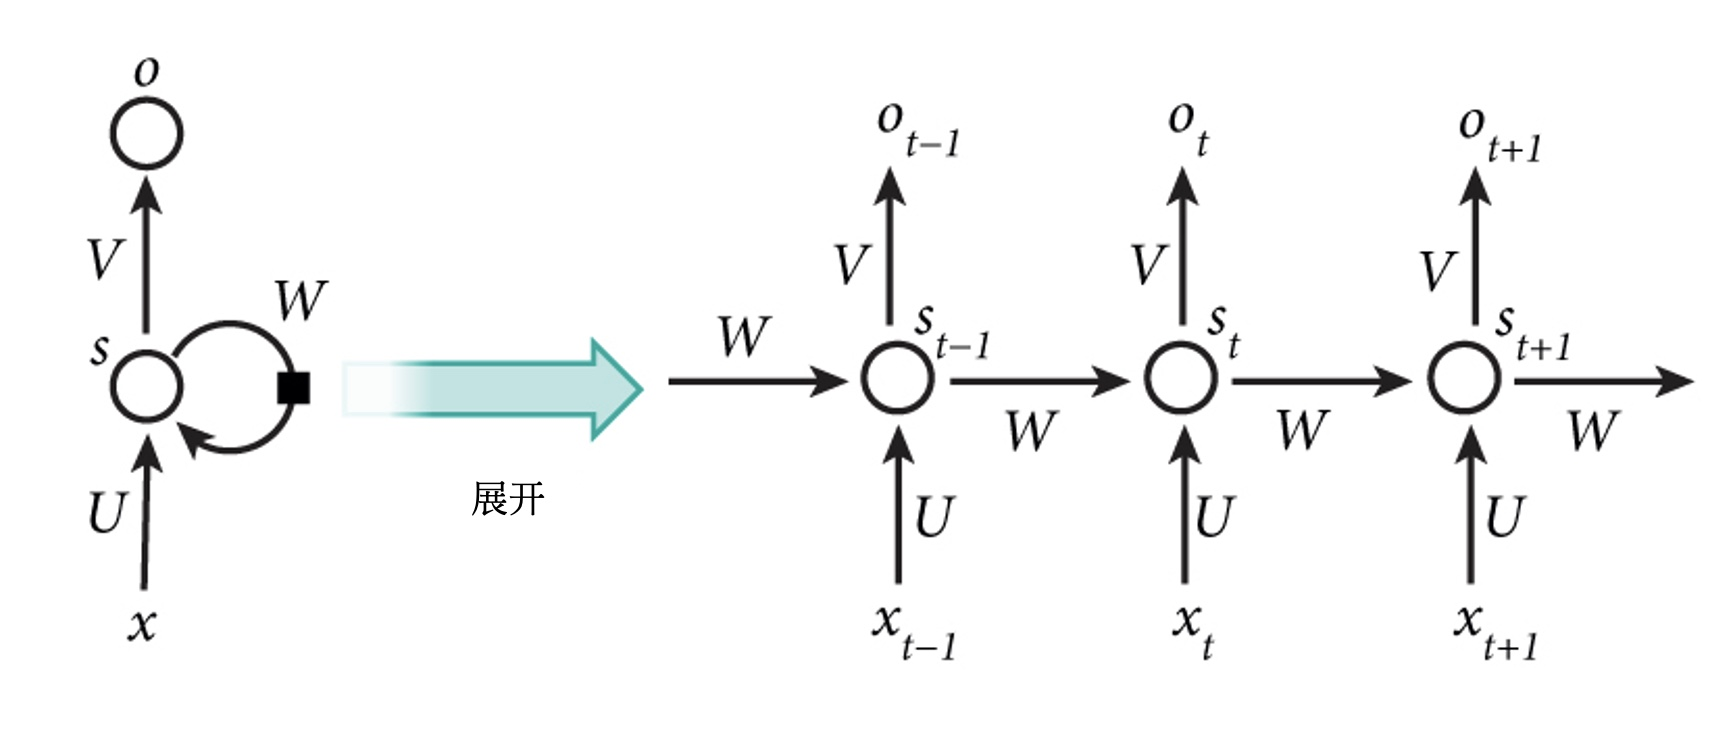
\includegraphics[width=0.6\linewidth]{循环神经网络.jpg}
    \caption{循环神经网络}
    \label{fig:循环神经网络}
  \end{figure}
该图显示了一个循环神经网络被展开成一个完整的神经网络。例如,如果输入序列是一个由5个单词组成的句子,那么网络就会被展开成一个5层神经网络,每个单词一层。这个网络在t时刻接收到输入 $x_t$ 之后,隐藏层的值是 $s_t$ ,输出值是 $o_t$ 。关键一点是, $x_t$ 的值不仅仅取决于 $s_t$ ,还取决于 $s_{t-1}$ 。
  用公式表示如下:
  \begin{equation}
      \begin{aligned}
          O_t &= g(V\cdot S_t) \\
          S_t &= f(U\cdot X_t + W\cdot S_{t-1})
      \end{aligned}
  \end{equation}

  $x_t$表示第$t$步的输入,例如$x_1$表示时刻1的特征向量。$s_t$表示第t步隐藏层状态,也就是网络中的“记忆”。$s_t$是由前一层的隐藏层状态和当前层的输入计算得到。函数$f(\cdot)$通常是一个非线性函数,如tanh或者ReLU。

\subsection{LSTM}
普通RNN有不能处理长依赖的问题,因此Hochreiter提出了一种长短期记忆网络-LSTM,以及它的变种,它是一种特殊的RNN,适用于学习长期依赖。现在LSTM已经被广泛应用于各个领域。

所有RNN都具有链式形式。在普通的RNN中,这种循环是一种非常简单的结构,比如简单的tanh层。
\begin{figure}
    \centering
    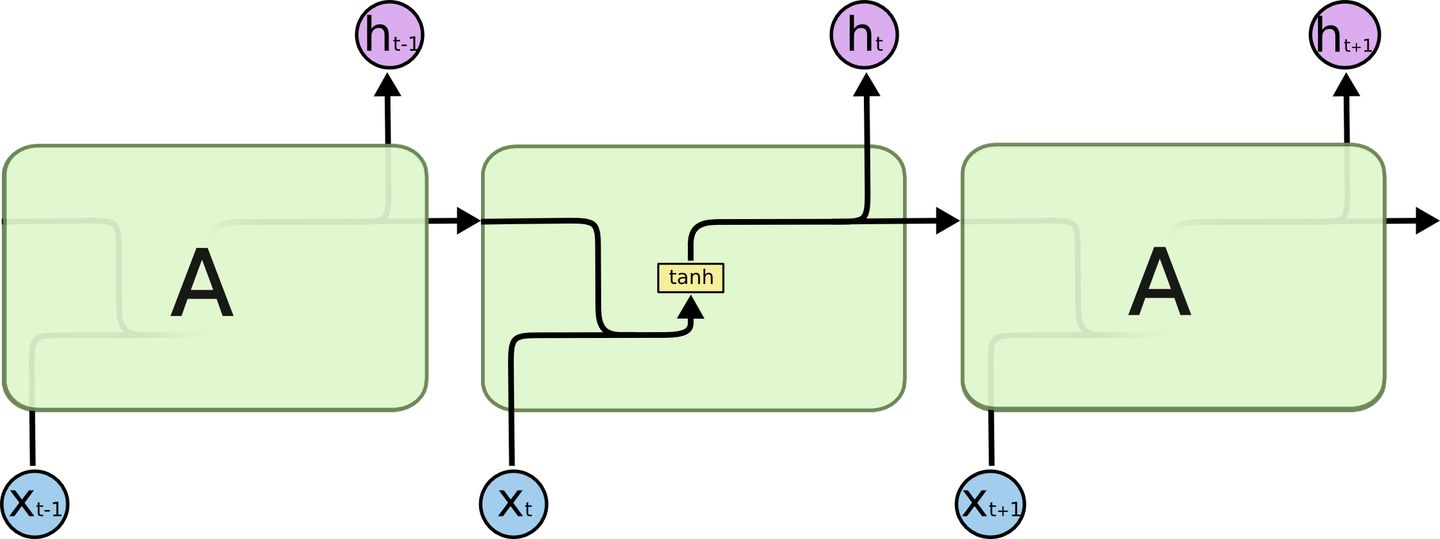
\includegraphics[width=0.6\linewidth]{普通RNN结构.jpg}
    \caption{普通RNN结构}
    \label{fig:普通RNN结构}
  \end{figure}

LSTM也具有这种链式结构,但循环单元里面不再是只有单一的神经网络层,而是构建了一些“门”(Gate)。原来的 RNN,由于这种链式结构的限制,很长的时刻以前的输入对现在的网络影响非常小,后向传播时那些梯度也很难影响很早以前的输入,即会出现梯度消失的问题。而 LSTM 通过构建“门”,让网络能记住那些非常重要的信息,比如遗忘门,来选择性清空过去的记忆和更新较新的信息。
\begin{figure}
    \centering
    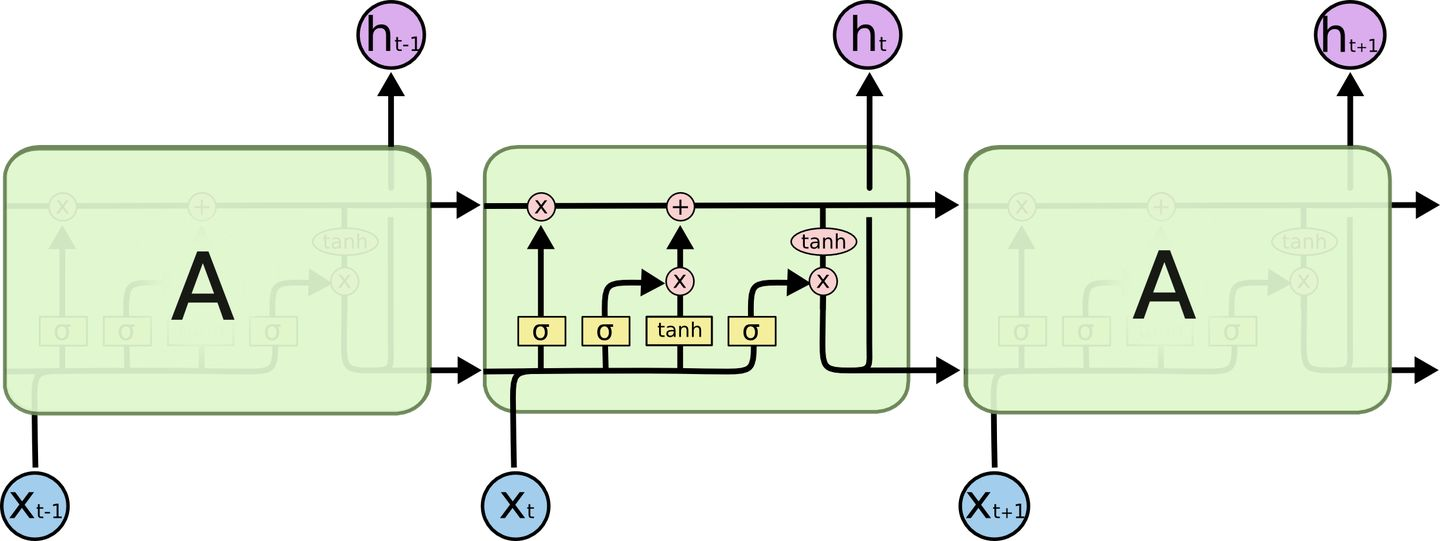
\includegraphics[width=0.6\linewidth]{LSTM结构.jpg}
    \caption{LSTM结构}
    \label{fig:LSTM结构}
  \end{figure}
  LSTM 中的第一步是决定从单元状态中丢弃什么信息。通过加入一个称为忘记门的$\sigma$层完成。遗忘门会读取上一时刻的输出$h_{t-1}$和当前时刻的输入$x_t$,计算出一个维度为n的向量$f_t$,该向量的值均在$(0, 1)$之间。1 表示“完全保留”上个神经元的状态信息,0 表示“完全舍弃”。

\begin{equation}
    \begin{aligned}
        f_t = \sigma(W_f\cdot x_t + U_f\cdot h_{t-1} + b_f)
    \end{aligned}
\end{equation}

下一步是确定该神经元的哪些新状态信息被存放在单元状态中。这里包含两个部分。第一,sigmoid 层,即 “输入门层” ,决定LSTM单元将更新哪些值。然后, tanh 层创建一个新的候选值$z_t$的向量,该向量可以加入到下一层单元状态中。

\begin{equation}
    \begin{aligned}
        i_t = \sigma(W_i\cdot[h_{t-1},x_t] + b_i)
    \end{aligned}
\end{equation}

\begin{equation}
    \begin{aligned}
        \widetilde {C_t} = tanh(W_C\cdot[h_{t-1},x_t]+b_C)
    \end{aligned}
\end{equation}
最后一步是将旧单元状态$c_{t-1}$更新为新状态$c_t$。把旧状态与遗忘门$f_t$相乘,丢弃掉之前需要丢弃的信息。接着与新状态进行相加。综合得出该神经元的输出的状态,也即更新单元的状态。
\begin{equation}
    \begin{aligned}
        C_t = f_t * C_{t-1} + i_t * \widetilde{C_t}
    \end{aligned}
\end{equation}

\subsection{GRU}
循环门单元(Gated Recurrent Unit,GRU),由 Cho, et al. (2014)提出。它组合了遗忘门和输入门到一个单独的“更新门”中。它也合并了cell state和hidden state,并且做了一些其他的改变。结果模型比标准LSTM模型更简单,
\begin{figure}
    \centering
    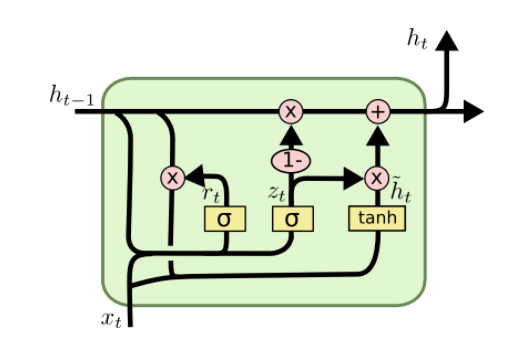
\includegraphics[width=0.6\linewidth]{GRU结构.png}
    \caption{GRU结构}
    \label{fig:GRU结构}
  \end{figure}

  \begin{equation}
    \begin{aligned}
        z_t = \sigma(W_z\cdot [h_{t-1},x_t])
    \end{aligned}
\end{equation}

\begin{equation}
    \begin{aligned}
        r_t = \sigma(W_r\cdot[h_{t-1},x_t])
    \end{aligned}
\end{equation}

\begin{equation}
    \begin{aligned}
        \widetilde {h_t} = tanh(W\cdot[r_t * h_{t-1}, x_t])
    \end{aligned}
\end{equation}

\begin{equation}
    \begin{aligned}
        h_t = (1- z_t) * h_{t-1} + z_t * \widetilde{h_t}
    \end{aligned}
\end{equation}

\section{基于图结构的RNN}
有向权重图$G=(V,E,W)$,$V$表示特征节点的集合,其中$|V|=N$, $E$表示特征间的关联关系,即图中的边,$W∈R[N*N]$为特征节点的相似度的加权邻接矩阵。将流量表示为G的一个图信号,P为每个节点特征数,则-时间t观察到的图信号。那么流量预测目的就是:给定G下,学得一个函数将T'个历史图信号映射到未来T时刻的图信号:
\begin{equation}
    h[X^{t-T+1}, X^{t-T+2},...,X^{t}; G] \Rightarrow [X^{t+1}, X^{t+2}, ..., X^{t+T}]
\end{equation}






% 循环神经网络解决了这个问题。它们是带有循环的网络,允许信息持续存在。循环神经网络可以被认为是同一个网络的多个副本,每个副本都会向后继者传递信息。
\section{实验方案设计及实验流程}


\section{算法性能评估}

其中多分类任务的准确率指标为对于每个标签,分别计算precision,然后取不加权平均。

\begin{table*}[t]
    \small
    \caption{部分评估结果,待填充具体数值}
    \label{table2}
    \centering
    \begin{tabular}{c|c|ccc|ccc|cc}
    \toprule
    
     数据集 &  任务  &  
     LR &  NB & DT & CNN & CNN-LSTM & GRU & DCRNN-A & DCRNN-B \\
    \midrule
    % & 5\% & 79.87 & 80.61 & 79.08 & 81.69 & 78.05 & 75.80 & 82.21 & \textbf{82.49}\\
    
    % & 4\% &79.35 & 80.22 & 78.89 & 80.85 & 75.07 & 72.41 & 82.11 & \textbf{82.44} \\
    
    UNSW-NB15 & 二分类 & 0.848 & 79.33 & 78.52 &  80.51 & 62.74 & 68.91 & \textbf{82.69} & 81.66 \\ 
    
    & 多分类 &76.73 & 77.96 & 76.82 & 77.98 & 47.11 & 56.30 & \textbf{81.05} & 79.94 \\
    
    % & 1\% & 66.58 & 70.09 & 68.18 & 71.23 & 32.95 & 46.71 & \textbf{71.76} & 71.62 \\
    \midrule
    % & 5\%& 70.55 & 69.41 & 68.40 &  71.45 & 70.72 & 65.11 & 71.24 &  \textbf{71.89} \\
    % & 4\% & 69.11 & 68.33& 67.13 & 70.37 & 70.41 & 64.61 & 69.74 & \textbf{71.10} \\
    NSL-KDD & 二分类 & 68.26 & 67.11 & 65.54 & 70.18 & 65.04 & 58.49 & 70.26 & \textbf{70.88} \\
    & 多分类 & 67.01 & 67.37 & 66.41 & 68.31 & 56.16 & 53.18 & 68.47 & \textbf{70.24} \\
    % & 1\% & 60.08 & 61.39 & 61.25 & 63.25 & 30.28 & 49.57 & 62.21 & \textbf{64.91} \\
    \midrule
    % & 0.5\%& 82.18 & 80.01 & 81.32 &  78.25 & \textbf{82.73} & 78.97 & 82.17 & 80.70\\
    % & 0.4\%& 80.85 & 79.09 & 79.82 & 76.32 & 81.53 &  75.86 & \textbf{81.70} & 79.92\\
    CAMPUS & 二分类 & 79.98 & 77.95 & 79.51 & 75.62 & 79.80 & 75.25 & \textbf{80.69} & 79.10\\
    & 多分类 & 76.33 & 77.01 & 77.54 & 73.01 & 76.59 & 59.28 & 78.12 & \textbf{78.89}\\
    % & 0.1\% & 69.21 & 70.99 & 71.42 & 67.92 & 42.46 & 55.92 & 72.23 & \textbf{73.17}\\
    
     \bottomrule
    
    \end{tabular}
    \end{table*}

\subsection{基于开源数据集的检测结果}

\subsection{基于真实数据的检测结果}

\chapter{流量检测系统的设计与实现}

\section{引言}

\section{使用大数据平台应对大规模流量的必要性}

\section{基于流式处理的实时检测模块}

\section{系统效率分析}
